%
% flocker.tex
% @author Sidharth Mishra
% @description 
% @copyright  BSD 3-Clause License
%
% Copyright (c) 2018, Sidharth Mishra
% All rights reserved.
%
% Redistribution and use in source and binary forms, with or without
% modification, are permitted provided that the following conditions are met:
%
% * Redistributions of source code must retain the above copyright notice, this
%  list of conditions and the following disclaimer.
%
% * Redistributions in binary form must reproduce the above copyright notice,
%  this list of conditions and the following disclaimer in the documentation
%  and/or other materials provided with the distribution.
%
% * Neither the name of the copyright holder nor the names of its
%  contributors may be used to endorse or promote products derived from
%  this software without specific prior written permission.
%
% THIS SOFTWARE IS PROVIDED BY THE COPYRIGHT HOLDERS AND CONTRIBUTORS "AS IS"
% AND ANY EXPRESS OR IMPLIED WARRANTIES, INCLUDING, BUT NOT LIMITED TO, THE
% IMPLIED WARRANTIES OF MERCHANTABILITY AND FITNESS FOR A PARTICULAR PURPOSE ARE
% DISCLAIMED. IN NO EVENT SHALL THE COPYRIGHT HOLDER OR CONTRIBUTORS BE LIABLE
% FOR ANY DIRECT, INDIRECT, INCIDENTAL, SPECIAL, EXEMPLARY, OR CONSEQUENTIAL
% DAMAGES (INCLUDING, BUT NOT LIMITED TO, PROCUREMENT OF SUBSTITUTE GOODS OR
% SERVICES; LOSS OF USE, DATA, OR PROFITS; OR BUSINESS INTERRUPTION) HOWEVER
% CAUSED AND ON ANY THEORY OF LIABILITY, WHETHER IN CONTRACT, STRICT LIABILITY,
% OR TORT (INCLUDING NEGLIGENCE OR OTHERWISE) ARISING IN ANY WAY OUT OF THE USE
% OF THIS SOFTWARE, EVEN IF ADVISED OF THE POSSIBILITY OF SUCH DAMAGE.
%
% @created Sat Mar 31 2018 22:05:54 GMT-0700 (PDT)
% @last-modified Mon Apr 02 2018 17:22:42 GMT-0700 (PDT)
%


\documentclass[../main]{subfiles}

\begin{document}

\section{Flocker}
\label{flocker}

{\em Flocker} \cite{flockerApp} is the core visualization component of the {\em flocking} simulation. It has been implemented using the p5.js\cite{p5js} Javascript library.

The source-code \cite{flockerSrc} for {\em flocker} has been written in \mbox{Typescript}~(TS) \cite{ts} which has been compiled and bundled into a single \code{.js} file using the \mbox{Webpack} tool \cite{wbpack}.

The central idea for implementing a simulation involving agents is coming up with a model for each agent. In our case, the agents -- {\em swallows} -- are {\em plain old Javascript objects} (POJO). Each swallow is given an \code{image}, \code{position}, \code{velocity}, and \code{acceleration}. The \code{image} is a \code{.PNG} image file of a swallow bird; \code{position}, \code{velocity}, and \code{acceleration} are p5.js \code{Vectors}. When a swallow spawns -- gets added to the simulation -- it is assigned a random position. Similarly, each swallow is assigned a random \code{velocity} in a random direction. However, initially, each swallow has zero \code{acceleration} -- no forces are acting on the swallow. Furthermore, internally each swallow has a {\em 4 x 4 matrix} to keep track of its position, scaling, and rotation. This matrix has been designed to be similar to {\em openframework's} \code{ofMatrix4x4} but, with utility methods specific to {\em flocker} like applications.

In our simulation, there are three types of forces acting on a swallow: {\em cohesion}, {\em separation}, and {\em alignment}. When the swallow flies, for each tick, the \code{acceleration} is the the aggregate of these three forces. Assuming each swallow to be of unit mass, using the equation \code{F = ma}, we can get \code{F = a}. The resultant \code{acceleration} updates the swallow's \code{velocity} which in turn modifies the swallow's \code{position}. The direction of the swallow's movement is determined from its \code{velocity}.

Since, there are three forces acting on a swallow influencing its flight behavior, we expose their desired strength and weights to the end user. The end user has the ability to modify the strength and weights of these forces to influence the behavior of the swallows and visualize the {\em flocking behavior}. The design choice for the user-interface (UI) will be covered in the next section \ref{flockerUI}.

{\em Note}: We use the words {\em neighborhood} --- {\em simulation space}, and {\em peer} --- {\em neighbor} interchangeably while talking about the computation of the three steering forces acting on the swallow.

\subsection{Swallow}
\label{swallow}

\begin{figure}
	\centering
	
\includegraphics[scale=0.15]{resources/swallow.png}
	\caption{The image used for a swallow.}
	\label{swallowImg}
\end{figure}

The {\em swallow} [Fig. \ref{swallowImg}] is the bird chosen for this simulation. The design was inspired by the exhibit at the {\em Exploratorium, San Francisco} named {\em Flock} \cite{jillflock}. The image however is a \code{.PNG} file created from a screenshot of an icon by Prahlad \cite{apSwallow}.

The swallow is designed to be an agent represented as a POJO that is intelligent enough to navigate through the environment and exhibit the flocking behavior according to the three forces.

\subsubsection{Separation}
\label{separation}

{\em Separation} is the force acting on a swallow that enables it to maintain a certain separation from its peers in the simulation space. It is a kind of collision prevention mechanism. Initially, each swallow starts with a desired separation strength of 50 units and the weight of this separation force is 3 units. Each swallow computes the steering separation force after taking into account its distance from all of its peers in the simulation space -- it is exhaustive. Once the steering force has been computed, the force acts on the swallow changing its acceleration causing it to stay clear of its peers in the simulation. The separation steering force algorithm [Fig. \ref{separationLogic}] shows how the separation force is computed for the swallow. It is based on the algorithms in \cite{reynolds1999steering, danshiffman}.

\begin{figure}
	\begin{verbatim}
Swallow::separation :: () -> Vector

1 steer = {0, 0} // the steering force
2 count = 0 // nbr of peers to clear
3 for each peer in simulation_space:
4   d = distance_between(me, peer)
5   if d > 0 and d < desired_separation:
6     diff = my_position - peer_position
7     steer = steer + 
        normalized_and_weighted_by_d(diff)
8     count = count + 1
9 if count > 0 then
    steer = steer / count
10 if |steer| > 0:
11  steer = normalize(steer)
12  steer = steer * max_velocity
13  steer = steer - my_velocity
14  steer = steer.limit(max_acceleration)
15 return steer
    \end{verbatim}
	\caption{Algorithm for computing the separation steering force.}
	\label{separationLogic}
\end{figure}

\begin{figure}
    \centering
	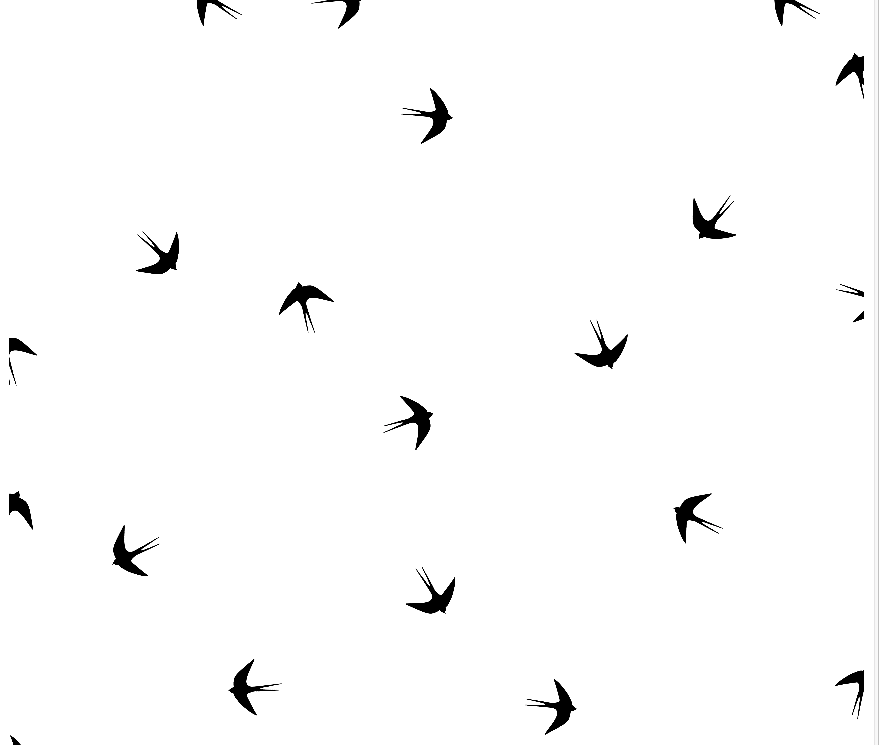
\includegraphics[scale=0.30, width=250pt]{resources/flocker_max_separation.png}
	\caption{Max separation simulation.}
	\label{maxSeparationImg}
\end{figure}

\subsubsection{Alignment}
\label{alignment}

{\em Alignment} is the force acting on a swallow that enables it to align itself with its peers in the simulation space.
When the swallow aligns itself, it moves in the same direction with the same velocity as its peers. Initially, each swallow starts with a desired alignment strength of 50 units and the weight of this alignment force is 2 units. Each swallow computes the steering alignment force after computing the average velocity of all its peers. This enables it to move in the same direction. This too like separation \ref{separation} is exhaustive. The alignment steering force algorithm [Fig. \ref{alignmentLogic}] shows how the alignment force is computed for the swallow. It too is based on the algorithms in \cite{reynolds1999steering, danshiffman}.

\begin{figure}
	\begin{verbatim}
Swallow::alignment :: () -> Vector

1 steer = {0, 0} // the steering force
2 sum = {0, 0} // cumulative velocities
3 count = 0 // peer count
4 for each peer in simulation_space:
5   d = distance_between(me, peer)
6   if d > 0 and d < desired_alignment:
7     sum = sum + my_velocity
8     count = count + 1
9 if count > 0:
10  sum = sum / count
11  sum = normalize(sum)
12  sum = sum * max_velocity
13  steer = sum - my_velocity
14  steer = steer.limit(max_acceleration)
15 return steer
    \end{verbatim}
	\caption{Algorithm for computing the alignment steering force.}
	\label{alignmentLogic}
\end{figure}

\begin{figure}
    \centering
	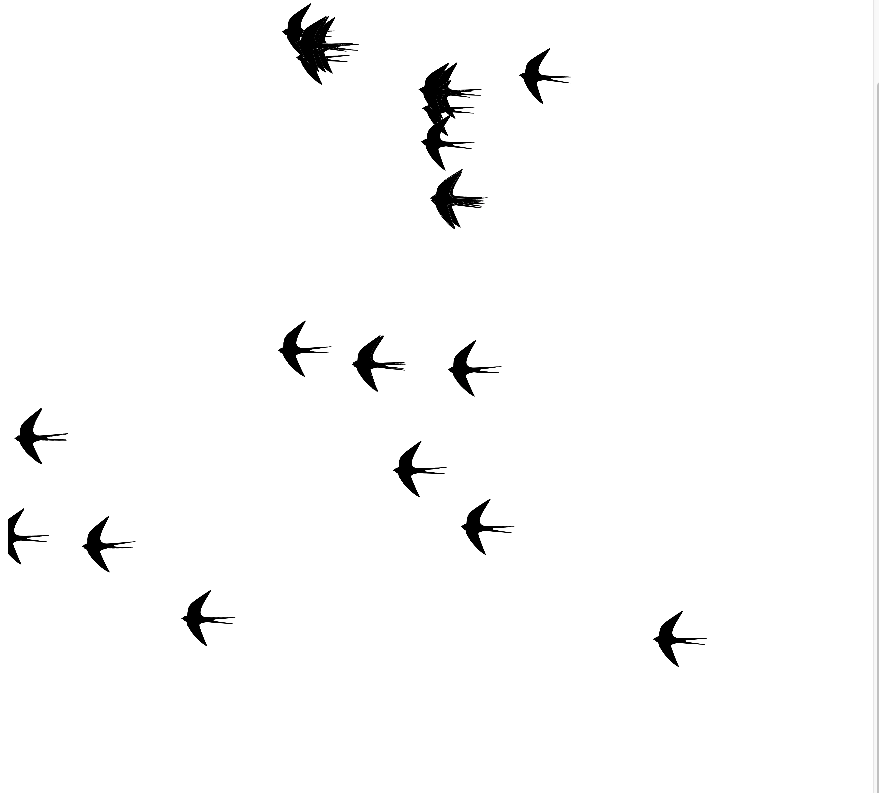
\includegraphics[scale=0.30, width=250pt]{resources/flocker_max_alignment.png}
	\caption{Max alignment simulation.}
	\label{maxAlignmentImg}
\end{figure}

\subsubsection{Cohesion}
\label{cohesion}

{\em Cohesion} is the force acting on a swallow that enables it to group together with its peers in the simulation space. This force steers the swallow towards its peers so that it can approach its peers and form a group -- flock.
In a sense, it can be considered as the gravitational force pulling in the swallows. Initially, each swallow starts with a desired cohesion strength of 50 units and the weight of this cohesion force is 2 units. Each swallow computes the steering cohesion force after computing the average position of all its peers. Then, the swallow moves towards this average position -- the center of gravity of the simulation space. This too like separation \ref{separation}, and alignment \ref{alignment} is exhaustive. The cohesion steering force algorithm [Fig. \ref{cohesionLogic}] shows how the cohesion force is computed for the swallow. It too is based on the algorithms in \cite{reynolds1999steering, danshiffman}.

\begin{figure}
	\begin{verbatim}
Swallow::cohesion :: () -> Vector

1 steer = {0, 0} // the steering force
2 sum = {0, 0} // cumulative positions
3 count = 0 // peer count
4 for each peer in simulation_space:
5   d = distance_between(me, peer)
6   if d > 0 and d < desired_cohesion:
7     sum = sum + peer_position
8     count = count + 1
9 if count > 0:
10  sum = sum / count
11  steer = seek(sum) // seek and apply
15 return steer

Swallow::seek :: (target: Vector) -> Vector

1 desired_position = target - my_position
2 desired_position = 
    normalize(desired_position)
3 steering_force = 
    desired_position * max_velocity
4 steering_force = 
    steering_force - my_velocity
5 steering_force = steering_force
    .limit(max_acceleration)
6 return steering_force
    \end{verbatim}
	\caption{Algorithm for computing the cohesion steering force.}
	\label{cohesionLogic}
\end{figure}

\begin{figure}
    \centering
	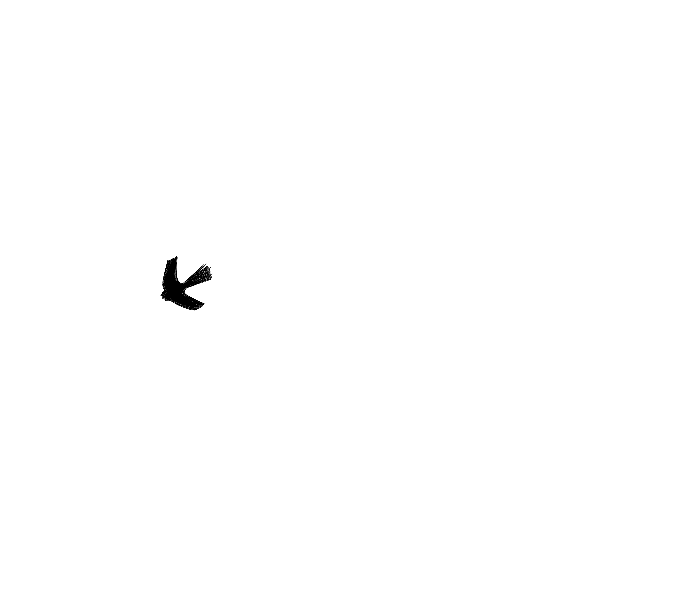
\includegraphics[scale=0.30, width=250pt]{resources/flocker_max_cohesion.png}
	\caption{Max cohesion simulation.}
	\label{maxCohesionImg}
\end{figure}

\subsection{Flocker and p5.js}
\label{flocker_p5js}

The entire simulation runs inside a HTML \code{canvas} element which is generated by the p5.js library. We generate the canvas with the same dimensions as the content area of our webpage -- the canvas is re-rendered when the window resizes. Furthermore, we make the simulation wrap around the edges so that the swallows do not fall off the viewable area -- the direction of motion and velocity are preserved when wrapping around, only the position is affected.

By default, the simulation caps the acceleration to a maximum value of \code{0.03}, and the velocity to a maximum value of \code{2.0}. This prevents the swallows from moving too fast and produces a smooth motion. The simulation starts out with \code{30} swallows, all at randomly generated positions. The user has the ability to add in a new swallow to the simulation by clicking on any area of the canvas. The new swallow is added at the point of mouse click but, with random velocity and direction~--~~to keep the motion random.

{\em Flocker} core has been designed as a standalone \mbox{library} that can be plugged in into different UI/view layer \mbox{implementations}. Comparing it with a traditional \mbox{\em model-view-controller} (MVC) architecture, the core would consist of the {\em model}, and the {\em controller} layers. Our UI is strictly restricted to the {\em view} layer only.

\end{document}